\section{Lego Mindstorms NXT}\label{lego:mindstorms-nxt}
I dette kapitel vil den valgte platform, \legoms, blive kort beskrevet med en begrundelse for dette valg.
Yderligere vil der blive argumenteret for valg af API til NXT-enheden.

\subsection{Hvad er Lego Mindstorms?}
\legoms er et byggesæt, hvor det er muligt at bygge programmerbare robotter i \lego-klodser.

Til at bygge disse robotter er der i \legoms nogle sensorer og aktuatorer. Sensorerne gør det muligt for robotten at modtage input fra sine omgivelser.
Ved brug af aktuatorerne kan robotten reagere på disse inputs.

Ud over de originale \lego dele er der også tredjeparts forhandlere, som har et udbud af andre sensorer og aktuatorer. \thilemann{Enten bør denne linje fjernes, eller også skal vi skrive om sådanne sensorer?}

\subsubsection{Hvad er NXT?}
Denne sektion er baseret på \cite{nxt}, hvilket omhandler NXT 2.0, som er den version der bruges i dette projekt.
NXT Intelligent Brick (oftest kaldt blot 'NXT' eller 'brick') er hjernen i \legoms robotten.
Det er den der står for at modtage og behandle input fra sensorer samt styre de monterede aktuatorer.
Et billede af NXT 2.0 kan ses i \cref{platform:nxt}.

\begin{figure}
\begin{center}
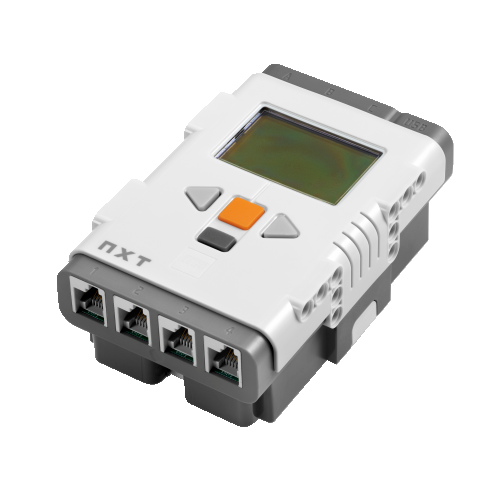
\includegraphics[scale=.5]{./graphics/nxt/brick}
\end{center}
\caption{'NXT Intelligent Brick'}
\label{platform:nxt}
\end{figure}

\subsubsection{Porte}
NXT'en har 3 motor porte (kaldet A, B og C) og 4 sensor porte (kaldet 1, 2, 3 og 4).

\subsubsection{Tilslutningsmuligheder}
Der kan kommunikeres med NXT'en ved at tilslutte den til en anden enhed med USB-kabel eller Bluetooth\textregistered.

\subsubsection{Feedback}
Til output har NXT'en en 100 x 64 pixel LCD display samt en 8 kHz højttaler.

\subsubsection{Styring}
NXT'en kan styres på to måder:
Man kan sende kommandoer og modtage beskeder (for eksempel sensor aflæsninger) på en ekstern enhed (oftest en computer eller en anden NXT).
Alternativt kan programmer sendes (via Bluetooth eller USB) til NXT'en, hvorfra de kan køres direkte, uafhængig af eksterne enheder.


\subsubsection{Tekniske specifikationer}
De tekniske specifikationer for NXT 2.0 kan ses på \cref{mindstorms:tekniske_spec} \cite{nxt}. 


\begin{figure}
\begin{tabular}{|c |c|}
\hline
Microcontroller & \shortstack{\\32-bit ARM7 microcontroller\\ 8-bit AVR controller}\\
\hline
RAM & \shortstack{ \\256 Kb FLASH, 64 Kb RAM \\ 4 Kb FLASH, 512 b RAM} \\
\hline
Kommuniation & \shortstack{ \\Bluetooth (Bluetooth Class II V2.0 compliant) \\ USB full speed port (12 Mbit/s)}\\
\hline
Input porte & 4 \\
\hline
Output porte & 3 \\
\hline
Display & 100 x 64 pixel LCD \\
\hline
Højttaler & 8 kHz lyd. 8-bit lydkanal og 2-16 kHz sample rate\\
\hline
Strømkilde & 6 AA batteries\\
\hline
\end{tabular}
\caption{LEGO MINDSTORMS NXT tekniske specifikationer}
\label{mindstorms:tekniske_spec}
\end{figure}


\subsection{Hvorfor LEGO MINDSTORMS NXT?}
Der er mange gode grunde til at vælge \legoms NXT.
Her er givet fire overordnede punkter, der vil blive gennemgået efterfølgende:

\begin{itemize}
\item{Tilgængelighed}
\item{Nemt at gå til}
\item{Stort udvalg af sensorer}
\item{Mange muligheder ift. styring}
\end{itemize}

\subsubsection{Tilgængelighed}
Grundet at \lego (inkl. \legoms) er ment til almindelige brugere, er det masseproduceret og kan derved købes forholdsvist billigt og i helt almindelige butikker (legetøjsforretninger og ofte også supermarkeder).

\subsubsection{Nemt at gå til}
Det faktum at man bygger sin robot i \lego klodser, med tilføjelse af \legoms sensorer/aktautorer gør det nemt at lave en konstruktion og derefter modificere den så den udfører sin opgave tilfredsstillende.

Denne høje versatilitet gør at \lego er perfekt til en prototype-orienteret fremgangsmåde for bygning af robotter.

\subsubsection{Stort udvalg af sensorer}
På grund af det store udvalg af sensorer kan man bygge robotter der kan løse et væld af opgaver.
Ved et projekt med høj usikkerhed, er det derved også nemt og billigt at udskifte en sensor.

\subsubsection{Mange muligheder ift. styring}
Her menes der både overordnet den måde hvorpå robotten styres, men især også den måde hvorpå NXT'en styres.
NXT'en kan udstyres med brugerdefineret firmware, der giver utroligt mange muligheder (og dermed også fleksibilitet) ift. hvordan den kan styres.

I afsnittet herefter vil der blive argumenteret for valg af API, hvor API her skal forstås som måden hvorpå robotten skal styres.

\section{Valg af NXT API}\label{nxt_api}
Den ideelle løsning ville være at vælge et system, hvor robotten styrer alt; både navigation og indsamling af sensor-målinger og selve kortlægningsdelen.
Dog er der begrænset med plads til data på NXT'en (256 KB flash, 64 KB RAM), samtidig med at dens regnekraft heller ikke er så god (32-bit ARM7 microcontroller).

Grundet disse begrænsninger og givet problemet der skal løses, ville der sagtens kunne laves et to-delt system.
Den ene del bestående af selve robotten, som skal navigere sig rundt i verden og bruge sine sensorer til at opfatte verden omkring sig.
Den anden del, som består af selve kortlægningen, kræver mere plads til data, samt større beregningskraft.
\mikael{Der skal nævnes noget i forhold til valg af PC og Kinect-afhængighed}

\subsubsection*{Overordnet valg}
For at kunne overholde ovenstående, skal der kunne laves et to-delt stykke software, hvor den ene del kører på robotten og den anden del på en stærkere platform, i vores tilfælde en PC.

Det der så skal vælges nu, er hvordan det software der skal køre på robotten skal laves, samt det software der skal køres på PC'en.
Vigtigt er at det skal være muligt for den ene del at kommunikere med den anden, da der skal kunne sendes kommandoer til robotten fra PC'en, samt at PC'en skal kunne modtage sensor-input fra robottten.

\subsubsection*{NXC}
Til det software der skal køres på robotten har vi valgt NXC, da det er simpelt og dækker alle behov.
NXC-programmer skrives i et C-lignende sprog, hvorefter disse programmer kan sendes til NXT'en og køres direkte der på.
Der er også stor mulighed for kommunikation mellem NXC-programmer og eksterne programmer.
Dette gør det muligt at skrive et program til NXC'en, hvorefter der kan udføres forskellige handlinger afhængig af hvad PC'en beder den om.
Der vil blive gået mere i dybden med NXC i \cref{nxc}.

\subsubsection*{MindSqualls}
Til det software der skal køres på PC, altså det der skal sørge for selve opdateringen og beregningen af kort, har vi valgt \mindsqualls.
\mindsqualls er et .NET bibliotek skrevet i \csharp, hvori det er muligt at kommunikere med en NXT, både ved at sende direkte kommandoer eller via abstraktion over NXTens aktuatorer/sensorer opfattet som objekter.
Valget faldt på \mindsqualls da dette var simpelt og dækkede alle behov ift. kommunikation med NXT.
Desuden har gruppen stor erfaring med \csharp og Visual Studio, hvilket også syntes værende en stor fordel.
\mindsqualls vil blive uddybet i \cref{mindsqualls}.
